\documentclass[pra,12pt]{revtex4}
\usepackage{amsmath}
\usepackage{amssymb}
\usepackage{graphicx}
\usepackage{color}
\usepackage{mathrsfs}
\usepackage{enumerate}
\usepackage{epigraph}
\usepackage{framed}
\usepackage[pdfborder={0 0 0},colorlinks=true,linkcolor=blue,urlcolor=blue]{hyperref}

\def\ket#1{\left|#1\right\rangle}
\def\bra#1{\left\langle#1\right|}
\def\braket#1{\left\langle#1\right\rangle}

\usepackage{fancyhdr}
\fancyhf{}
\lhead{\tiny Y.~D.~Chong}
\rhead{\scriptsize PH4401: Quantum Mechanics III}
\lfoot{}
\rfoot{\thepage}
\pagestyle{fancy}

\setlength{\parindent}{14pt}
\renewcommand{\theequation}{5.\arabic{equation}}

\renewcommand{\baselinestretch}{1.0}
\setlength{\parskip}{0.04in}
\setlength{\epigraphwidth}{.6\textwidth}

\def\thesection{5.\arabic{section}}
\def\thesubsection{5.\arabic{section}.\arabic{subsection}}

\begin{document}
\setcounter{page}{87}

\begin{center}
{\Large \textbf{Chapter 5: Quantum Electrodynamics}}
\end{center}

%% \epigraph{From so simple a beginning
%%  endless forms most beautiful and most wonderful
%%  have been, and are being, evolved.}{Charles Darwin,
%%   \textit{The Origin of Species}}

This chapter gives an introduction to \textbf{quantum
  electrodynamics}, the quantum theory of the electromagnetic field
and its interactions with electrons and other charged particles.  We
begin by formulating a quantum Hamiltonian for an electron in a
classical electromagnetic field.  Then we study how to quantize
Maxwell's equations, arriving at a quantum field theory in which the
elementary excitations are photons---particles of light.  The final
step is to formulate a theory in which electrons and photons are
treated on the same quantum mechanical footing, as excitations of
underlying quantum fields.  Along the way, we will see how relativity
can be accomodated with quantum theory.

Quantum electrodynamics is an extremely rich and intricate theory, and
we will leave out many important topics.  Interested readers are
referred to are Dyson's 1951 lecture notes on quantum electrodynamics
[\ref{cite:dyson}], and Zee's textbook \textit{Quantum Field Theory in
  a Nutshell} [\ref{cite:zee}].

\section{Quantization of the Lorentz Force Law}

\subsection{Non-relativistic electrons in an electromagnetic field}
\label{sec:nonrel}

Consider a non-relativistic charged particle in an electromagnetic
field.  As we are mainly interested in the physics of electrons
interacting with electromagnetic fields, we henceforth take the
electric charge of the particle to be $-e$, where $e =
1.602\times10^{-19}\,\mathrm{C}$ is the elementary charge.  To
describe particles with an arbitrary electric charge $q$, simply
perform the substitution $e \rightarrow -q$ in the formulas you will
subsequently encounter.

We wish to formulate the Hamiltonian governing the quantum dynamics of
such a particle, subject to two simplifying assumptions: (i) the
particle has charge and mass but is otherwise ``featureless'' (i.e.,
we ignore the spin angular momentum and magnetic dipole moment that
real electrons possess), and (ii) the electromagnetic field is treated
as a classical field, meaning that the electric and magnetic fields
are definite quantities rather than operators.  (We will see how to go
beyond these simplifications later.)

Classically, the electromagnetic field acts on the particle via the
Lorentz force law,
\begin{equation}
  \mathbf{F}(\mathbf{r},t) = -e\Big(\mathbf{E}(\mathbf{r},t)
  + \dot{\mathbf{r}}\times \mathbf{B}(\mathbf{r},t)\Big),
\end{equation}
where $\mathbf{r}$ and $\dot{\mathbf{r}}$ denote the position and
velocity of the particle, $t$ is the time, and $\mathbf{E}$ and
$\mathbf{B}$ are the electric and magnetic fields.  If no other forces
are present, Newton's second law yields the equation of motion
\begin{equation}
  m\ddot{\mathbf{r}} = -e\Big(\mathbf{E}(\mathbf{r},t)
  + \dot{\mathbf{r}} \times \mathbf{B}(\mathbf{r},t)\Big),
  \label{eom}
\end{equation}
where $m$ is the particle's mass.  To quantize this, we must first
convert the equation of motion into the form of Hamilton's equations
of motion.

Let us introduce the electromagnetic scalar and vector potentials
$\Phi(\mathbf{r},t)$ and $\mathbf{A}(\mathbf{r},t)$:
\begin{align}
  \mathbf{E}(\mathbf{r},t) &= - \nabla \Phi(\mathbf{r},t) - \frac{\partial\mathbf{A}}{\partial t}, \\
  \mathbf{B}(\mathbf{r},t) &= \nabla \times \mathbf{A}(\mathbf{r},t).
  \label{Bfield}
\end{align}
We now postulate that the equation of motion \eqref{eom} can be
described by the Lagrangian
\begin{framed}
\begin{equation}
  L(\mathbf{r},\dot{\mathbf{r}},t) = \frac{1}{2}m\dot{\mathbf{r}}^2
  + e \Big[\Phi(\mathbf{r},t) - \dot{\mathbf{r}} \cdot \mathbf{A}(\mathbf{r},t)
    \Big].
  \label{Lag}
\end{equation}
\end{framed}
\vskip -0.15in
\noindent
This follows the usual prescription for the Lagrangian as kinetic
energy minus potential energy, with $-e\Phi$ serving as the potential
energy function, except for the $-e\dot{\mathbf{r}} \cdot \mathbf{A}$
term.  To see if this Lagrangian works, plug it into the
Euler-Lagrange equations
\begin{equation}
  \frac{\partial L}{\partial r_i} = \frac{d}{dt}
  \frac{\partial L}{\partial \dot{r}_i}.
  \label{EulerLagrange}
\end{equation}
The partial derivatives of the Lagrangian are:
\begin{align}
  \begin{aligned}
    \frac{\partial L}{\partial r_i} &=
    e\Big[\partial_i \Phi - \dot{r}_j \,\partial_i A_j \Big]\\
    \frac{\partial L}{\partial \dot{r}_i} &= m\dot{r}_i - e A_i.
  \end{aligned}
\end{align}
Now we want to take the \textit{total} time derivative of $\partial L
/\partial \dot{r}_i$.  In doing so, note that the $\mathbf{A}$ field
has its own $t$-dependence, as well as varying with the particle's
$t$-dependent position.  Thus,
\begin{align}
  \begin{aligned}
    \frac{d}{dt} \frac{\partial L}{\partial \dot{r}_i}
    &= m\ddot{r}_i - e\, \frac{d}{dt} A_i(\mathbf{r}(t),t) \\
    &= m\ddot{r}_i - e\, \partial_t A_i
    - e\, \dot{r}_j \partial_j A_i.
  \end{aligned}
\end{align}
(In the above equations, $\partial_i \equiv \partial/\partial r_i$,
where $r_i$ is the $i$-th component of the position vector, while
$\partial_t \equiv \partial/\partial t$.)  Plugging these expressions
into the Euler-Lagrange equations \eqref{EulerLagrange} gives
\begin{align}
  \begin{aligned}
    m\ddot{r}_i &=
    -e\Big[\Big(-\partial_i \Phi - \partial_t A_i\Big)
      + \dot{r}_j \Big( \partial_i A_j - \partial_j A_i\Big) \Big] \\
    &= -e \Big[E_i(\mathbf{r},t) + \big(\dot{\mathbf{r}} \times
      \mathbf{B}(\mathbf{r},t) \big)_i\, \Big].
  \end{aligned}
\end{align}
(The last step can be derived by expressing the cross product using
the Levi-Cevita symbol, and using the identity $\varepsilon_{ijk}
\varepsilon_{lmk} = \delta_{il} \delta_{jm} - \delta_{im}
\delta_{jl}$.)  This exactly matches Eq.~\eqref{eom}, as desired.

We now use the Lagrangian to derive the Hamiltonian.  The canonical
momentum is
\begin{equation}
  p_i = \frac{\partial L}{\partial \dot{r}_i} = m\dot{r}_i - e A_i.
  \label{canonp}
\end{equation}
The Hamiltonian is defined as $H(\mathbf{r},\mathbf{p}) = \mathbf{p}
\cdot \dot{\mathbf{r}} - L$.  Using Eq.~\eqref{canonp}, we express it
in terms of $\mathbf{p}$ rather than $\dot{\mathbf{r}}$:
\begin{align}
  \begin{aligned}
    H &= \mathbf{p}\cdot \left(\frac{\mathbf{p}+e\mathbf{A}}{m}\right)
    - \left(\frac{|\mathbf{p}+e\mathbf{A}|^2}{2m}
    + e\Phi - \frac{e}{m}(\mathbf{p}+e\mathbf{A})\cdot \mathbf{A}\right) \\
    &= \frac{|\mathbf{p}+e\mathbf{A}|^2}{m}
    - \frac{e}{m}\mathbf{A}\cdot \left(\mathbf{p}+e\mathbf{A}\right)
    - \left(\frac{|\mathbf{p}+e\mathbf{A}|^2}{2m}
    + e\Phi - \frac{e}{m}(\mathbf{p}+e\mathbf{A})\cdot \mathbf{A}\right).
  \end{aligned}
\end{align}
After cancelling various terms, we obtain
\begin{equation}
  H = \frac{|\mathbf{p}+e\mathbf{A}(\mathbf{r},t)|^2}{2m} - e\Phi(\mathbf{r},t).
  \label{H0}
\end{equation}
This looks a lot like the Hamiltonian for a non-relativistic particle
in a scalar potential,
\begin{equation*}
  H = \frac{|\mathbf{p}|^2}{2m} + V(\mathbf{r},t).
\end{equation*}
In Eq.~\eqref{H0}, the $-e\Phi$ term acts like a potential energy,
which is no surprise.  More interestingly, the vector potential
appears via the substitution
\begin{equation}
  \mathbf{p} \rightarrow \mathbf{p} + e\mathbf{A}(\mathbf{r},t).  
\end{equation}

What does this mean?  Think about what ``momentum'' means for a
charged particle in an electromagnetic field.  Noether's theorem
states that each symmetry of a system (whether classical or quantum)
is associated with a conservation law.  Momentum is the quantity
conserved when the system is symmetric under spatial translations.
One of Hamilton's equations states that
\begin{equation*}
  \frac{dp_i}{dt} = \frac{\partial H}{\partial r_i},
\end{equation*}
which implies that if $H$ is $\mathbf{r}$-independent, then
$d\mathbf{p}/dt = 0$.  But when the electromagnetic potentials are
$\mathbf{r}$-independent, the quantity $m\dot{\mathbf{r}}$ (which we
usually call momentum) is not necessarily conserved!  Take the
potentials
\begin{equation}
  \Phi(\mathbf{r}, t) = 0, \;\;\; \mathbf{A}(\mathbf{r}, t) = Ct \hat{z},
\end{equation}
where $C$ is some constant.  These potentials are
$\mathbf{r}$-independent, but the vector potential is time-dependent,
so the $-\dot{\mathbf{A}}$ term in Eq.~\eqref{Bfield} gives a
non-vanishing electric field:
\begin{equation}
  \mathbf{E}(\mathbf{r},t) = - C\hat{z}, \;\;\;\mathbf{B}(\mathbf{r},t) = 0.
\end{equation}
The Lorentz force law then says that
\begin{equation}
  \frac{d}{dt}(m\dot{\mathbf{r}}) = eC\hat{z},
\end{equation}
and thus $m\dot{\mathbf{r}}$ is not conserved.  On the other hand, the
quantity $\mathbf{p} = m\dot{\mathbf{r}} - e \mathbf{A}$ \textit{is}
conserved:
\begin{equation}
  \frac{d}{dt}(m\dot{\mathbf{r}} - e\mathbf{A}) =
  eC\hat{z} - eC\hat{z} = 0.
\end{equation}
Hence, this is the appropriate canonical momentum for a particle in an
electromagnetic field.

We are now ready to go from classical to quantum mechanics.  Replace
$\mathbf{r}$ with the position operator $\hat{\mathbf{r}}$, and
$\mathbf{p}$ with the momentum operator $\hat{\mathbf{p}}$.  The
resulting quantum Hamiltonian is
\begin{framed}
  \begin{equation}
    \hat{H}(t) = \frac{|\hat{\mathbf{p}}+e\mathbf{A}(\hat{\mathbf{r}},t)|^2}{2m}
    - e\Phi(\hat{\mathbf{r}},t).
    \label{quantumH}
  \end{equation}
\end{framed}
\vskip -0.15in
\noindent
Note: the momentum operator is $\hat{\mathbf{p}} = -i\hbar\nabla$
in the wavefunction representation, as usual.

\subsection{Gauge symmetry}
\label{sec:gauge}

The Hamiltonian \eqref{quantumH} possesses a subtle property known as
\textbf{gauge symmetry}.  Suppose we modify the scalar and vector
potentials via the substitutions
\begin{align}
  \Phi(\mathbf{r},t) &\rightarrow \Phi(\mathbf{r},t) - \dot{\Lambda}(\mathbf{r},t) \label{gauge-subst-1} \\
  \mathbf{A}(\mathbf{r},t) &\rightarrow
  \mathbf{A}(\mathbf{r},t) + \nabla{\Lambda}(\mathbf{r},t),
  \label{gauge-subst-2}
\end{align}
where $\Lambda(\mathbf{r},t)$ is an arbitrary scalar field called a
\textbf{gauge field}.  This is the \textbf{gauge transformation} of
classical electromagnetism, which as we know leaves the electric and
magnetic fields unchanged.  When applied to the Hamiltonian
\eqref{quantumH}, it generates a new Hamiltonian
\begin{equation}
  \hat{H}_\Lambda(t)
  = \frac{|\hat{\mathbf{p}}+e\mathbf{A}(\hat{\mathbf{r}},t) + e\nabla\Lambda(\hat{\mathbf{r}},t)|^2}{2m}
  - e\Phi(\hat{\mathbf{r}},t) + e\dot{\Lambda}(\hat{\mathbf{r}},t).
\end{equation}
Now suppose $\psi(\mathbf{r},t)$ is a wavefunction obeying the
Schr\"odinger equation for the original Hamiltonian $\hat{H}$:
\begin{equation}
  i\hbar\frac{\partial\psi}{\partial t} =
  \hat{H}(t) \psi(\mathbf{r},t)
  = \left[\frac{|\hat{\mathbf{p}}+e\mathbf{A}(\hat{\mathbf{r}},t)|^2}{2m}
  - e\Phi(\hat{\mathbf{r}},t) \right]\psi(\mathbf{r},t).
\end{equation}
Then it can be shown that the wavefunction $\psi\,
\exp(-ie\Lambda/\hbar)$ automatically satisfies the Schr\"odinger
equation for the transformed Hamiltonian $\hat{H}_\Lambda$:
\begin{equation}
  i\hbar\frac{\partial}{\partial t} \left[\psi(\mathbf{r},t) \, \exp\left(-\frac{ie\Lambda(\mathbf{r},t)}{\hbar}\right)\right] =
  \hat{H}_\Lambda(t) \left[\psi(\mathbf{r},t) \, \exp\left(-\frac{ie\Lambda(\mathbf{r},t)}{\hbar}\right)\right].
  \label{gaugeschrod}
\end{equation}

To prove this, observe how time and space derivatives act on the new
wavefunction:
\begin{align}
  \begin{aligned}
    \frac{\partial}{\partial t} \left[\psi \, \exp\left(-\frac{ie\Lambda}{\hbar}\right)\right] &=
    \left[\frac{\partial\psi}{\partial t} \;-\; \frac{ie}{\hbar} \dot{\Lambda}\, \psi
      \,\, \right] \exp\left(\frac{ie\Lambda}{\hbar}\right)\\
    \nabla \left[\psi \, \exp\left(-\frac{ie\Lambda}{\hbar}\right)\right] &=
    \left[\nabla \psi - \frac{ie}{\hbar} \nabla \Lambda \,\psi \right] \exp\left(\frac{ie\Lambda}{\hbar}\right).
  \end{aligned}
\end{align}
When the extra terms generated by the $\exp(ie\Lambda/\hbar)$ factor
are slotted into the Schr\"odinger equation, they cancel the gauge
terms in the scalar and vector potentials.  For example,
\begin{align}
  \Big(-i\hbar\nabla + e\mathbf{A} + e\nabla\Lambda\Big)
  \left[\psi \, \exp\left(-\frac{ie\Lambda}{\hbar}\right)\right] &=
  \Big[\left(-i\hbar\nabla + e\mathbf{A}\right)\psi\Big]\;
  \exp\left(-\frac{ie\Lambda}{\hbar}\right)
  \label{first_gauge_action}
\end{align}
If we apply the $(-i\hbar\nabla + e\mathbf{A} + e\nabla\Lambda)$
operator a second time, it has a similar effect but with the quantity
in square brackets on the right-hand side of
\eqref{first_gauge_action} taking the place of $\psi$:
\begin{equation}
  \Big|-i\hbar\nabla + e\mathbf{A} + e\nabla\Lambda\;\Big|^2
  \left[\psi \, \exp\left(-\frac{ie\Lambda}{\hbar}\right)\right]  
  =   \Big[\left|-i\hbar\nabla + e\mathbf{A}\right|^2\psi\Big]\;
  \exp\left(-\frac{ie\Lambda}{\hbar}\right).
\end{equation}
The remainder of the proof for Eq.~\eqref{gaugeschrod} can be carried
out straightforwardly.

The above result can be stated in a simpler form if the
electromagnetic fields are static.  In this case, the time-independent
electromagnetic Hamiltonian is
\begin{equation}
  \hat{H} = \frac{|\hat{\mathbf{p}}+e\mathbf{A}(\hat{\mathbf{r}})|^2}{2m}
  - e\Phi(\hat{\mathbf{r}}).
\end{equation}
Suppose $\hat{H}$ has eigenenergies $\{E_m \}$ and energy
eigenfunctions $\{\psi_m(\mathbf{r})\}$.  Then the gauge-transformed
Hamiltonian
\begin{equation}
  \hat{H}_\Lambda = \frac{|\hat{\mathbf{p}}+e\mathbf{A}(\hat{\mathbf{r}}) + e\nabla\Lambda(\mathbf{r})|^2}{2m}
  - e\Phi(\hat{\mathbf{r}})
\end{equation}
has the same energy spectrum $\{E_m\}$, with eigenfunctions
$\{\,\psi_m(\mathbf{r}) \exp[-ie\Lambda(\mathbf{r})/\hbar]\,\}$.

\subsection{The Aharonov-Bohm effect}

In quantum electrodynamics, it is the electromagnetic scalar and
vector potentials that appear directly in the Hamiltonian, not the
electric and magnetic fields.  This has profound consequences.  For
example, even if a charged quantum particle resides in a region with
zero magnetic field, it can feel the effect of nonzero \textit{vector
  potentials} produced by magnetic fluxes elsewhere in space, a
phenomenon called the \textbf{Aharonov-Bohm effect}.

A simple setting for observing the Aharonov-Bohm effect is shown in
the figure below.  A particle is trapped in a ring-shaped region (an
``annulus''), of radius $R$ and width $d \ll R$.  Outside the annulus,
we set $-e\Phi\rightarrow\infty$ so that the wavefunction vanishes;
inside the annulus, we set $\Phi = 0$.  We ignore the $z$-dependence
of all fields and wavefunctions, so that the problem is
two-dimensional.  We define polar coordinates $(r,\phi)$ with the
origin at the ring's center.

\begin{figure}[h]
  \centering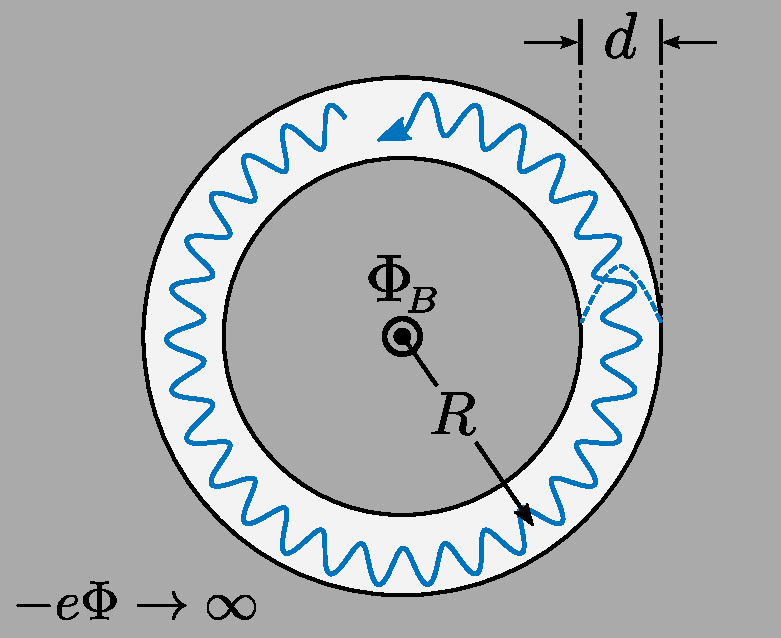
\includegraphics[width=0.32\textwidth]{annulus}
\end{figure}

Now, suppose we thread magnetic flux (e.g., using a solenoid) through
the origin, which lies in the region enclosed by the annulus.  This
flux can be described via the vector potential
\begin{equation}
  \mathbf{A}(r,\phi) = \frac{\Phi_B}{2\pi r} \, \mathbf{e}_\phi,
  \label{Asolenoid}
\end{equation}
where $\mathbf{e}_\phi$ is the unit vector pointing in the azimuthal
direction.  We can verify from Eq.~\eqref{Asolenoid} that the total
magnetic flux through any loop of radius $r$ enclosing the origin is
$(\Phi_B/2\pi r)(2\pi r) = \Phi_B$.  The fact that this is independent
of $r$ implies that the magnetic flux density is concentrated in an
infintesimal area surrounding the origin, and zero everywhere
else. However, the vector potential $\mathbf{A}$ is nonzero
everywhere.

The time-independent Schr\"odinger equation is
\begin{equation}
  \frac{1}{2m}\left|-i\hbar\nabla+
  \frac{e\Phi_B}{2\pi r} \, \mathbf{e}_\phi\right|^2 \psi(r,\phi)
  = E\psi(r,\phi),
  \label{ABschrod}
\end{equation}
with the boundary conditions $\psi(R\pm d/2,0) = 0$.  For sufficiently
large $R$, we can guess that the eigenfunctions have the form
\begin{equation}
  \psi(r,\phi) \approx
  \begin{cases}
  \psi_0 \, \cos\left(\frac{\pi}{d}(r-R)\right)\, e^{i k R \phi},
  & r \in [R-d/2, R + d/2] \\
  0 & \textrm{otherwise}.
  \end{cases}
\end{equation}
This describes a ``waveguide mode'' with a half-wavelength wave
profile in the $r$ direction (so as to vanish at $r = R \pm d/2$),
traveling in the azimuthal direction with wavenumber $k$.  The
normalization constant $\psi_0$ is unimportant.  We need the
wavefunction to be single-valued under a $2\pi$ variation in the
azimuthal coordinate, so
\begin{equation}
  k \cdot 2\pi R = 2\pi n \;\;\;\Rightarrow \;\;\; k = \frac{n}{R},
  \;\;\;\mathrm{where}\;\; n \in \mathbb{Z}.
\end{equation}
Plugging this into Eq.~\eqref{ABschrod} yields the energy levels
\begin{align}
  E_n &= \frac{1}{2m} \left[
    \left(\frac{n\hbar}{R} + \frac{e\Phi_B}{2\pi R}\right)^2
    + \left(\frac{\pi\hbar}{d}\right)^2 \right] \\
  &= \frac{e^2}{8\pi^2mR^2} \left(\Phi_B + \frac{nh}{e} \right)^2
  + \frac{\pi^2\hbar^2}{2md^2}.
  \label{abcurves}
\end{align}
These energy levels are sketched versus the magnetic flux $\Phi_B$ in
the figure below:

\begin{figure}[h]
  \centering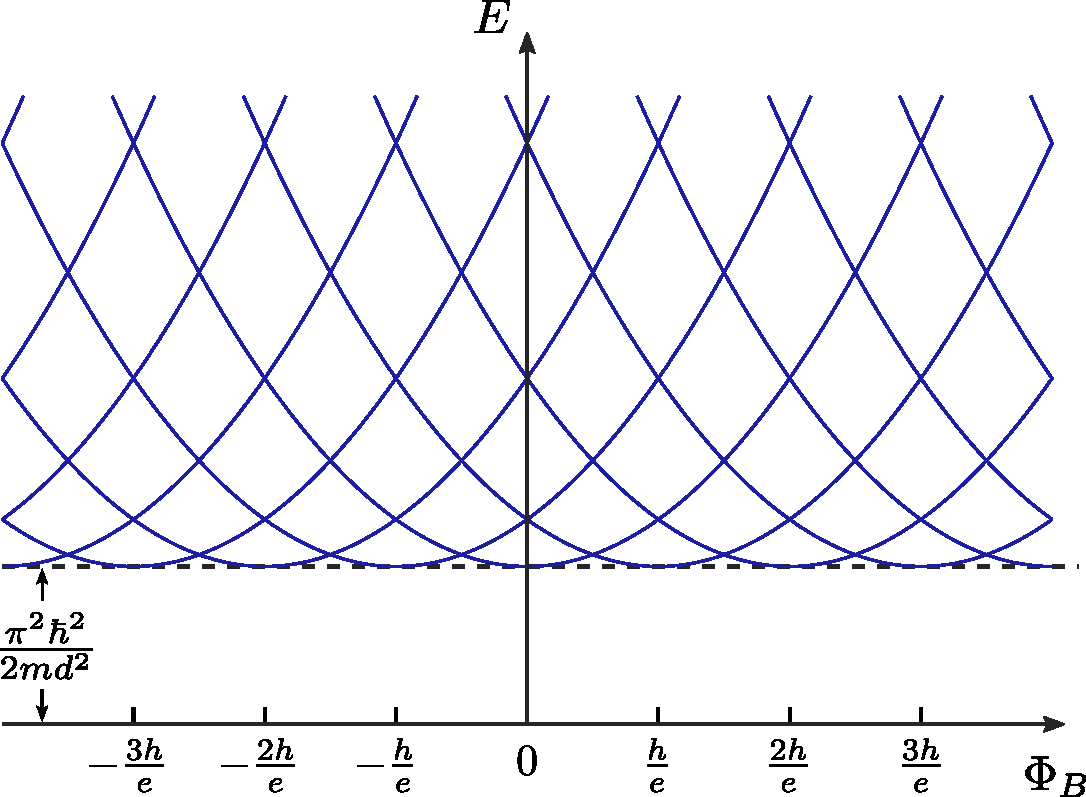
\includegraphics[width=0.55\textwidth]{abring}
\end{figure}

Each energy level has a quadratic dependence on $\Phi_B$.  Variations
in $\Phi_B$ affect the energy levels despite the fact that $\mathbf{B}
= 0$ in the annular region where the electron resides.  This is a
manifestation of the Aharonov-Bohm effect.

It is noteworthy that the curves of different $n$ are centered at
different values of $\Phi_B$ corresponding to multiples of $h/e =
4.13567\times10^{-5}\,\mathrm{T}\,\mathrm{m}^2$, a fundamental unit of
magnetic flux called the \textbf{magnetic flux quantum}.  In other
words, changing $\Phi_B$ by an exact multiple of $h/e$ leaves the
energy spectrum unchanged!  This invariance property, which does not
depend on the width of the annulus or any other geometrical parameters
of the system, can be explained using gauge symmetry.  When an extra
flux of $nh/e$ (where $n\in\mathbb{Z}$) is threaded through the
annulus, Eq.~\eqref{Asolenoid} tells us that the change in vector
potential is $\Delta \mathbf{A} = (n\hbar/ e r) \mathbf{e}_\phi$.  But
we can undo the effects of this via the gauge field
\begin{equation}
  \Lambda(r,\phi) = - \frac{n\hbar}{e} \, \phi \;\;\;\Rightarrow
  \begin{cases}\nabla \Lambda &= \displaystyle - (n\hbar/er) \, \mathbf{e}_\phi
    \\ \displaystyle e^{-ie\Lambda/\hbar} &= \displaystyle e^{in\phi}.
  \end{cases}
\end{equation}
Note that this $\Lambda$ is not single-valued, but that's not a
problem!  Both $\nabla\Lambda$ and the phase factor
$\exp(-ie\Lambda/\hbar)$ \textit{are} single-valued, and those are the
quantities that enter into the gauge symmetry relations
\eqref{gauge-subst-1}--\eqref{gauge-subst-2}.

\section{Dirac's Theory of the Electron}

\subsection{The Dirac Hamiltonian}
\label{sec:DiracH}

So far, we have been using $p^2/2m$-type Hamiltonians, which are
limited to describing non-relativistic particles.  In 1928, Paul Dirac
formulated a Hamiltonian that can describe electrons moving close to
the speed of light, thus successfully combining quantum theory with
special relativity. Another triumph of Dirac's theory is that it
accurately predicts the magnetic moment of the electron.

Dirac's theory begins from the time-dependent Schr\"odinger wave
equation,
\begin{equation}
  i\hbar\, \partial_t\, \psi(\mathbf{r},t)
  = \hat{H} \psi(\mathbf{r},t).
  \label{schrod}
\end{equation}
Note that the left side has a first-order time derivative.  On the
right, the Hamiltonian $\hat{H}$ contains spatial derivatives in the
form of momentum operators.  We know that time and space derivatives
of wavefunctions are related to energy and momentum by
\begin{equation}
    i\hbar\, \partial_t\; \leftrightarrow \;
    E, \qquad
    -i\hbar\, \partial_j \;\leftrightarrow \;
    p_j.
\end{equation}
We also know that the energy and momentum of a relativistic particle
are related by
\begin{equation}
  E^2 = m^2c^4 + \sum_{j=1}^3 p_j^2c^2,
  \label{Erelativistic}
\end{equation}
where $m$ is the rest mass and $c$ is the speed of light.  Note that
$E$ and $p$ appear to the same order in this equation.  (Following the
usual practice in relativity theory, we use Roman indices $j \in
\{1,2,3\}$ for the spatial coordinates $\{x,y,z\}$.)

Since the left side of the Schr\"odinger equation \eqref{schrod} has a
first-order time derivative, a relativistic Hamiltonian should involve
first-order spatial derivatives.  So we make the guess
\begin{equation}
  \hat{H} = \alpha_0 mc^2 + \sum_{j=1}^3 \alpha_j \hat{p}_j c,
  \label{Dirac0}
\end{equation}
where $\hat{p}_j \equiv -i\hbar \partial/\partial x_j$.  The $mc^2$
and $c$ factors are placed for later convenience.  We now need to
determine the dimensionless ``coefficients'' $\alpha_0$, $\alpha_1$,
$\alpha_2$, and $\alpha_3$.

For a wavefunction with definite momentum $\mathbf{p}$ and energy
$E$,
\begin{equation}
  \hat{H}\psi = E \psi \;\;\;\Rightarrow \;\;\;
  \left(\alpha_0mc^2 + \sum_{j=1}^3\alpha_j p_jc\right) \psi = E\,\psi.
\end{equation}
This is obtained by replacing the $\hat{p}_j$ operators with definite
numbers.  If $\psi$ is a scalar, this would imply that $\alpha_0 mc^2
+ \sum_{j}\alpha_j p_j c = E$ for certain scalar coefficients
$\{\alpha_0, \dots, \alpha_3\}$, which does not match the relativistic
energy-mass-momentum relation \eqref{Erelativistic}.

But we can get things to work if $\psi(\mathbf{r},t)$ is a
multi-component wavefunction, rather than a scalar wavefunction, and
the $\alpha$'s are matrices acting on those components via the
matrix-vector product operation.  In that case,
\begin{framed}
  \begin{equation}
    \hat{H} = \hat{\alpha}_0 mc^2 + \sum_{j=1}^3 \hat{\alpha}_j \hat{p}_j c,
    \;\; \mathrm{where}\;\; \hat{p}_j \equiv -i\hbar\, \partial_j,
    \label{Dirac}
  \end{equation}
\end{framed}
\vskip -0.15in
\noindent
where the hats on $\{\hat{\alpha}_0, \dots, \hat{\alpha}_3\}$ indicate
that they are matrix-valued.  Applying the Hamiltonian twice gives
\begin{equation}
  \left(\hat{\alpha}_0mc^2 + \sum_{j=1}^3\hat{\alpha}_j p_j c\right)^{\!2}\;
  \psi = E^2\,\psi.
\end{equation}
This can be satisfied if
\begin{equation}
  \left(\hat{\alpha}_0 mc^2 + \sum_{j=1}^3\hat{\alpha}_j p_j c\right)^2
  = E^2\, \hat{I},
\end{equation}
where $\hat{I}$ is the identity matrix.  Expanding the square (and
taking care of the fact that the $\hat{\alpha}_\mu$ matrices need not
commute) yields
\begin{equation}
  \hat{\alpha}_0^2 m^2c^4
  + \sum_j \left(\hat{\alpha}_0 \hat{\alpha}_j + \hat{\alpha}_j \hat{\alpha}_0\right) mc^3 p_j
  + \sum_{jj'} \hat{\alpha}_j \hat{\alpha}_{j'} \, p_j p_{j'} \,c^2 = E^2\hat{I}.
\end{equation}
This reduces to Eq.~\eqref{Erelativistic} if the $\hat{\alpha}_\mu$
matrices satisfy
\begin{align}
  \begin{aligned}
    \hat{\alpha}_\mu^2 &= \hat{I} \;\;\; \textrm{for} \;\;\mu=0,1,2,3,
    \;\;\textrm{and} \\
    \hat{\alpha}_\mu \hat{\alpha}_\nu
    + \hat{\alpha}_\nu \hat{\alpha}_\mu &= 0
    \;\;\; \textrm{for} \;\;\mu \ne \nu.
  \end{aligned}
\end{align}
(We use Greek symbols for indices ranging over the four spacetime
coordinates $\{0,1,2,3\}$.)  The above can be written more concisely
using the anticommutator:
\begin{equation}
  \{\hat{\alpha}_\mu, \hat{\alpha}_\nu\} = 2\delta_{\mu\nu},
  \;\;\; \textrm{for} \;\;\mu,\nu=0,1,2,3.
  \label{Dirac_anticomm}
\end{equation}
Also, we need the $\hat{\alpha}_\mu$ matrices to be Hermitian, so that
$\hat{H}$ is Hermitian.

It turns out that the smallest possible Hermitian matrices that can
satisfy Eq.~\eqref{Dirac_anticomm} are $4\times4$ matrices.  The
choice of matrices (or ``representation'') is not uniquely determined.
One particularly useful choice is called the \textbf{Dirac
  representation}:
\begin{align}
  \begin{aligned}
    \hat{\alpha}_0 &= \begin{bmatrix}
      \hat{I}\, & \hat{0} \\ \hat{0} & -\hat{I}
    \end{bmatrix}, \;\;\;
    \hat{\alpha}_1 = \begin{bmatrix}
      \hat{0} & \hat{\sigma}_1 \\ \hat{\sigma}_1 & \hat{0}
    \end{bmatrix} \\
    \hat{\alpha}_2 &= \begin{bmatrix}
      \hat{0} & \hat{\sigma}_2 \\ \hat{\sigma}_2 & \hat{0}
    \end{bmatrix}, \;\;\;
    \hat{\alpha}_3 = \begin{bmatrix}
      \hat{0} & \hat{\sigma}_3 \\ \hat{\sigma}_3 & \hat{0}
    \end{bmatrix},
  \end{aligned}
  \label{alpha_matrices}
\end{align}
where $\{\hat{\sigma}_{1}, \hat{\sigma}_{2}, \hat{\sigma}_{3}\}$
denote the usual Pauli matrices.  Since the $\hat{\alpha}_\mu$'s are
$4\times4$ matrices, it follows that $\psi(\mathbf{r})$ is a
four-component field.

\subsection{Eigenstates of the Dirac Hamiltonian}
\label{sec:deigenstates}

According to Eq.~\eqref{Erelativistic}, the energy eigenvalues of the
Dirac Hamiltonian are
\begin{equation}
  E = \pm \sqrt{m^2c^4 + \sum_{j} p_j^2c^2}.
\end{equation}
This is plotted below:

\begin{center}
  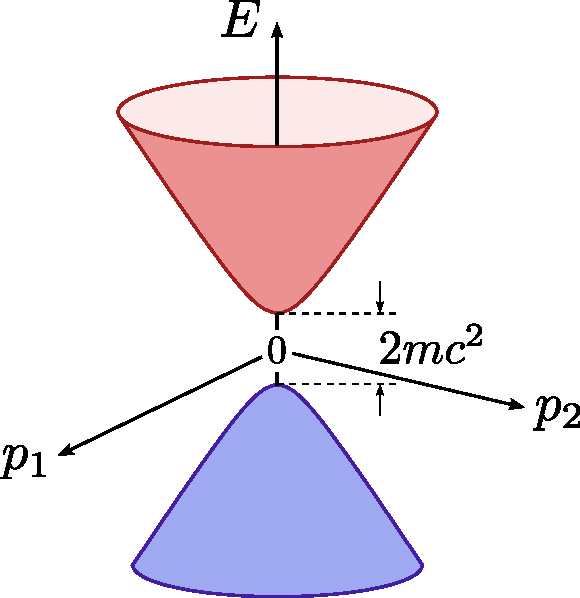
\includegraphics[width=0.27\textwidth]{diraccone}
\end{center}

\noindent
The energy spectrum forms two hyperbolic bands.  For each
$\mathbf{p}$, there are two degenerate positive energy eigenvalues,
and two degenerate negative energy eigenvalues, for a total of four
eigenvalues (matching the number of wavefunction components).  The
upper band matches the dispersion relation for a massive relativistic
particle, as desired.  But what about the negative-energy band?  Who
ordered that?

It might be possible for us to ignore the existence of the
negative-energy states, if we only ever consider an isolated electron;
we could just declare the positive-energy states to be the ones we are
interested in, and ignore the others.  However, the problem becomes
hard to dismiss once we let the electron interact with another system,
such as the electromagnetic field.  Under such circumstances, the
availability of negative-energy states extending down to $E\rightarrow
-\infty$ would destabilize the positive-energy electron states, since
the electron can repeatedly hop to states with ever more negative
energies by shedding energy (e.g., by emitting photons).  This is
obviously problematic.  However, let us wait for a while (till
Section~\ref{sec:positrons}) to discuss how the stability problem
might be resolved.

For now, let us take a closer look at the meaning of the Dirac
wavefunction.  Its four components represent a four-fold ``internal''
degree of freedom, distinct from the electron's ordinary kinematic
degrees of freedom.  Since there are two energy bands, the assignment
of an electron to the upper or lower band (or some superposition
thereof) consitutes two degrees of freedom.  Each band must then
posssess a two-fold degree of freedom (so that $2\times 2 = 4$), which
turns out to be associated with the electron's spin.

To see explicitly how this works, let us pick a representation for the
$\hat{\alpha}_\mu$ matrices.  The choice of representation determines
how the four degrees of freedom are encoded in the individual
wavefunction components.  We will use the Dirac representation
\eqref{alpha_matrices}.  In this case, it is convenient to divide the
components into upper and lower parts,
\begin{equation}
  \psi(\mathbf{r},t) = \begin{bmatrix}\psi_A(\mathbf{r},t)
    \\ \psi_B(\mathbf{r},t)
  \end{bmatrix},
\end{equation}
where $\psi_A$ and $\psi_B$ have two components each.  Then, for an
eigenstate with energy $E$ and momentum $\mathbf{p}$, applying
\eqref{alpha_matrices} to the Dirac equation \eqref{Dirac} gives
\begin{align}
  \psi_A &= \frac{1}{E - mc^2} \sum_j \hat{\sigma}_j p_j \psi_B,
  \label{dirac_nonrel1} \\
  \psi_B &= \frac{1}{E + mc^2} \sum_j \hat{\sigma}_j p_j \psi_A.
  \label{dirac_nonrel2}
\end{align}
Consider the non-relativistic limit, $|\mathbf{p}| \rightarrow 0$, for
which $E$ approaches either $mc^2$ or $-mc^2$.  For the upper band ($E
\gtrsim mc^2$), the vanishing of the denominator in
Eq.~\eqref{dirac_nonrel1} tells us that the wavefunction is dominated
by $\psi_A$.  Conversely, for the lower band ($E \lesssim -mc^2$),
Eq.~\eqref{dirac_nonrel2} tells us that the wavefunction is dominated
by $\psi_B$.  We can thus associate the upper ($A$) and lower ($B$)
components with the band degree of freedom.  Note, however, that this
is only an approximate association that holds in the non-relativistic
limit!  In the relativistic regime, upper-band states can have
non-vanishing values in the $B$ components, and vice versa.  (There
does exist a way to make the upper/lower spinor components correspond
rigorously to positive/negative energies, but this requires a more
complicated representation than the Dirac representation
[\ref{cite:foldy}].)

\subsection{Dirac electrons in an electromagnetic field}
\label{sec:diracem}

To continue pursuing our objective of interpreting the Dirac
wavefunction, we must determine how the electron interacts with an
electromagnetic field.  We introduce electromagnetism by following the
same procedure as in the non-relativistic theory
(Section~\ref{sec:nonrel}): add $-e\Phi(\mathbf{r},t)$ as a scalar
potential function, and add the vector potential via the substitution
\begin{equation}
  \hat{\mathbf{p}} \rightarrow \hat{\mathbf{p}}
  + e\mathbf{A}(\hat{\mathbf{r}},t).  
\end{equation}
Applying this recipe to the Dirac Hamiltonian (\ref{Dirac}) yields
\begin{equation}
  i\hbar \, \partial_t \psi
  = \left\{\hat{\alpha}_0 mc^2 -e\Phi(\mathbf{r},t)
  + \sum_{j} \hat{\alpha}_j \Big[-i\hbar\,\partial_j
    +eA_j(\mathbf{r},t) \Big] c\right\}\psi(\mathbf{r},t).
  \label{DiracEM}
\end{equation}
You can check that this has the same gauge symmetry properties as the
non-relativistic theory discussed in Section~\ref{sec:gauge}.

In the Dirac representation \eqref{alpha_matrices},
Eq.~\eqref{DiracEM} reduces to
\begin{align}
  i\hbar\, \partial_t \, \psi_A
  &= \big(+mc^2 -e\Phi \big)\,
  \psi_A
  \,+\, \sum_{j} \hat{\sigma}_j \big(-i\hbar\partial_j
    +eA_j \big) \,c\;\psi_B \label{Dirac2a} \\
  i\hbar\, \partial_t \, \psi_B
  &= \big(- mc^2 -e\Phi\big)\,
  \psi_B \,+\, \sum_{j} \hat{\sigma}_j \big(-i\hbar\partial_j
    +eA_j \big)\, c\;\psi_A, \label{Dirac2b}
\end{align}
where $\psi_A$ and $\psi_B$ are the previously-introduced
two-component objects corresponding to the upper and lower halves of
the Dirac wavefunction.

In the non-relativistic limit, solutions to the above equations can be
cast in the form
\begin{align}
  \begin{aligned}
  \psi_{A}(\mathbf{r},t) &= \Psi_{A}(\mathbf{r},t)\,
  \exp\left[-i\left(\frac{mc^2}{\hbar}\right)t\right] \\
  \psi_{B}(\mathbf{r},t) &= \Psi_{B}(\mathbf{r},t)\,
  \exp\left[-i\left(\frac{mc^2}{\hbar}\right)t\right].
  \end{aligned}
\end{align}
The exponentials on the right side are the $\exp(-i\omega t)$ factor
corresponding to the rest energy $mc^2$, which dominates the
electron's energy in the non-relativistic limit.  (Note that by using
$+mc^2$ rather than $-mc^2$, we are explicitly referencing the
positive-energy band.)  If the electron is in an eigenstate with
$\mathbf{p} = 0$ and there are no electromagnetic fields, $\Psi_A$ and
$\Psi_B$ would just be constants.  Now suppose the electron is
non-relativistic but not in a $\mathbf{p} = 0$ eigenstate, and the
electromagnetic fields are weak but not necessarily vanishing.  In
that case, $\Psi_A$ and $\Psi_B$ are functions that vary with $t$, but
slowly.

Plugging this ansatz into Eqs.~\eqref{Dirac2a}--\eqref{Dirac2b} gives
\begin{align}
  i\hbar\, \partial_t \, \Psi_A
  &= -e\Phi\; \Psi_A
  \,+\, \sum_{j} \hat{\sigma}_j \big(-i\hbar\partial_j
    +eA_j \big) c\;\Psi_B \label{Dirac3a} \\
  \big(i\hbar\, \partial_t \, + 2mc^2 + e\Phi\big)
  \Psi_B
  &= \sum_{j} \hat{\sigma}_j \big(-i\hbar\partial_j
    +eA_j \big) c\;\Psi_A. \label{Dirac3b}
\end{align}
On the left side of Eq.~\eqref{Dirac3b}, the $2mc^2$ term dominates
over the other two, so
\begin{equation}
  \Psi_B \;\approx\; \frac{1}{2mc}\, \sum_{j}
  \hat{\sigma}_j \big(-i\hbar\partial_j +eA_j \big) \;\Psi_A.
\end{equation}
Plugging this into Eq.~\eqref{Dirac3a} yields
\begin{equation}
  i\hbar\, \partial_t \, \Psi_A
  = \left\{-e\Phi \,+\, \frac{1}{2m} \sum_{jk} \hat{\sigma}_j \hat{\sigma}_k
  \big(-i\hbar\partial_j +eA_j \big)
  \big(-i\hbar\partial_k +eA_k \big) \right\}\;\Psi_A.
\end{equation}
Using the identity $\hat{\sigma}_j\hat{\sigma}_k = \delta_{jk}\hat{I}
+ i \sum_i \varepsilon_{ijk}\sigma_i$:
\begin{align}
  \begin{aligned}
  i\hbar\, \partial_t \, \Psi_A
  &= \Bigg\{-e\Phi
  \,+\, \frac{1}{2m} \big|-i\hbar\nabla +e\mathbf{A} \big|^2 \\
  &\qquad+\, \frac{i}{2m} \sum_{ijk} \varepsilon_{ijk} \hat{\sigma}_i
  \big(-i\hbar\partial_j +eA_j \big)
  \big(-i\hbar\partial_k +eA_k \big)
  \Bigg\} \Psi_A.
  \end{aligned}
\end{align}
Look carefully at the last term in the curly brackets.  Expanding the
square yields
\begin{equation*}
  \frac{i}{2m}\sum_{ijk}\varepsilon_{ijk}\hat{\sigma}_i
  \Big(-\partial_j\partial_k -i\hbar e \partial_jA_k
  - i\hbar e \big[A_k\partial_j + A_j\partial_k \big]
  + e^2A_jA_k \Big).
\end{equation*}
Due to the antisymmetry of $\varepsilon_{ijk}$, all terms inside the
parentheses that are symmetric under $j$ and $k$ cancel out when
summed over.  The only survivor is the second term, which gives
\begin{equation}
  \frac{\hbar e}{2m}\sum_{ijk}\varepsilon_{ijk}\hat{\sigma}_i
  \partial_jA_k = \frac{\hbar e}{2m} \hat{\boldsymbol{\sigma}}
  \,\cdot\, \mathbf{B}(\mathbf{r},t),
\end{equation}
where $\mathbf{B} = \nabla\times\mathbf{A}$ is the magnetic field.
Hence,
\begin{equation}
  i\hbar\, \partial_t \, \Psi_A
  = \left\{-e\Phi
  \,+\, \frac{1}{2m} \big|-i\hbar\nabla +e\mathbf{A} \big|^2
  \,-\, \left(-\frac{\hbar e}{2m}\, \hat{\boldsymbol{\sigma}}\right)
  \,\cdot\, \mathbf{B} \right\} \Psi_A.
\end{equation}
This is an exact match for Eq.~\eqref{quantumH}, except that the
Hamiltonian has an additional term of the form $-
\hat{\boldsymbol{\mu}} \cdot \hat{\mathbf{B}}$.  This additional term
corresponds to the potential energy of a magnetic dipole of moment
$\boldsymbol{\mu}$ in a magnetic field $\mathbf{B}$.  The Dirac theory
therefore predicts the electron's magnetic dipole moment to be
\begin{equation}
  |\boldsymbol{\mu}| = \frac{\hbar e}{2m}.
  \label{Diracmu}
\end{equation}
Remarkably, this matches the experimentally-observed magnetic dipole
moment to about one part in $10^3$.  The residual mismatch between
Eq.~\eqref{Diracmu} and the actual magnetic dipole moment of the
electron is understood to arise from quantum fluctuations of the
electronic and electromagnetic quantum fields.  Using the full theory
of quantum electrodynamics, that ``anomalous magnetic moment'' can
also be calculated and matches experiment to around one part in
$10^9$, making it one of the most precise theoretical predictions in
physics!  For details, see Ref.~[\ref{cite:zee}].

It is noteworthy that we did not set out to include spin in the
theory, yet it arose, seemingly unavoidably, as a by-product of
formulating a relativistic theory of the electron.  This is a
manifestation of the general principle that relativistic quantum
theory is more constrained than non-relativistic quantum
theory~[\ref{cite:dyson}].  Due to the demands imposed by relativistic
symmetries, spin is not allowed to be an optional part of the theory
of the relativistic electron---it has to be built into the theory at a
fundamental level.

\subsection{Positrons and Dirac Field Theory}
\label{sec:positrons}

As noted in Section~\ref{sec:deigenstates}, the stability of the
quantum states described by the Dirac equation is threatened by the
presence of negative-energy solutions.  To get around this problem,
Dirac suggested that what we regard as the ``vacuum'' may actually be
a state, called the \textbf{Dirac sea}, in which all negative-energy
states are occupied.  Since electrons are fermions, the Pauli
exclusion principle would then forbid decay into the negative-energy
states, stabilizing the positive-energy states.

At first blush, the idea seems ridiculous; how can the vacuum contain
an infinite number of particles?  However, we shall see that the idea
becomes more plausible if the Dirac equation is reinterpreted as a
single-particle \textit{construction} which arises from a more
fundamental quantum field theory.  The Dirac sea idea is an inherently
multi-particle concept, and we know from Chapter 4 that quantum field
theory is a natural framework for describing multi-particle quantum
states.  Let us therefore develop this theory.

Consider again the eigenstates of the single-particle Dirac
Hamiltonian with definite momenta and energies.  Denote the
positive-energy wavefunctions by
\begin{equation}
  \frac{u_{\mathbf{k}\sigma} \, e^{i\mathbf{k}\cdot \mathbf{r}}}{(2\pi)^{3/2}}
  = \langle \mathbf{r} | \mathbf{k}, +, \sigma\rangle,
  \quad\mathrm{where}\;\;
  \hat{H} |\mathbf{k}, +, \sigma\rangle
  = \epsilon_{\mathbf{k}\sigma} |\mathbf{k}, +, \sigma\rangle.
  \label{Diraces1}
\end{equation}
The negative-energy wavefunctions are
\begin{equation}
  \frac{v_{\mathbf{k}\sigma} \, e^{-i\mathbf{k}\cdot \mathbf{r}}}{(2\pi)^{3/2}}
  = \langle \mathbf{r} | \mathbf{k}, -, \sigma\rangle,
  \quad\mathrm{where}\;\;
  \hat{H} |\mathbf{k}, -, \sigma\rangle
  = - \epsilon_{\mathbf{k}\sigma} |\mathbf{k}, -, \sigma\rangle.
  \label{Diraces2}
\end{equation}
Note that $|\mathbf{k}, -, \sigma\rangle$ denotes a negative-energy
eigenstate with momentum $-\hbar\mathbf{k}$, not $\hbar\mathbf{k}$.
The reason for this notation, which uses different symbols to label
the positive-energy and negative-energy states, will become clear
later.  Each of the $u_{\mathbf{k}\sigma}$ and $v_{\mathbf{k}\sigma}$
terms are four-component objects (spinors), and for any given
$\mathbf{k}$, the set
\begin{equation*}
  \{ u_{\mathbf{k}\sigma}, v_{\mathbf{k},\sigma}\;\;  | \;\; \sigma = 1,2  \}
\end{equation*}
forms an orthonormal basis for the four-dimensional spinor space.
Thus,
\begin{equation}
  \sum_{n} \left(u^n_{\mathbf{k}\sigma}\right)^* u^n_{\mathbf{k}\sigma'} = \delta_{\sigma\sigma'}, \;\;
  \sum_{n} \left(u^n_{\mathbf{k}\sigma}\right)^* v^n_{\mathbf{k}\sigma'} = 0, \;\;
  \textrm{etc.}
  \label{uvorthog}
\end{equation}
Here we use the notation where $u^n_{\mathbf{k}\sigma}$ is the $n$-th
component of the $u_{\mathbf{k}\sigma}$ spinor, and likewise for the
$v$'s.

Following the second quantization procedure from Chapter 4, let us
introduce a fermionic Fock space $\mathscr{H}_F$, as well as a set of
creation/annihilation operators:
\begin{align*}
  \hat{b}_{\mathbf{k}\sigma}^\dagger \;\; \mathrm{and} \;\; \hat{b}_{\mathbf{k}\sigma}
  &\;\;\mathrm{create/annihilate} \;\; |\mathbf{k}, +, \sigma\rangle\\
  \hat{d}_{\mathbf{k}\sigma}^\dagger \;\; \mathrm{and} \;\; \hat{d}_{\mathbf{k}\sigma}
  &\;\;\mathrm{create/annihilate} \;\; |\mathbf{k}, -, \sigma\rangle.
\end{align*}
These obey the fermionic anticommutation relations
\begin{align}
  \begin{aligned}
    \{\hat{b}_{\mathbf{k}\sigma}, \hat{b}_{\mathbf{k}'\sigma'}^\dagger \}
    = \delta^3(\mathbf{k}-\mathbf{k}') \, \delta_{\sigma\sigma'}, \quad
    \{\hat{d}_{\mathbf{k}\sigma}, \hat{d}_{\mathbf{k}'\sigma'}^\dagger \}
    = \delta^3(\mathbf{k}-\mathbf{k}') \, \delta_{\sigma\sigma'} \\
    \{\hat{b}_{\mathbf{k}\sigma}, \hat{b}_{\mathbf{k}'\sigma'} \} = 
    \{\hat{b}_{\mathbf{k}\sigma}, \hat{d}_{\mathbf{k}'\sigma'} \} = 
    \{\hat{d}_{\mathbf{k}\sigma}, \hat{d}_{\mathbf{k}'\sigma'} \} = 0, \;\;\textrm{etc.}
  \end{aligned}
  \label{Diracanticommutation0}
\end{align}
The Hamiltonian is
\begin{equation}
  \hat{H} = \int d^3k \sum_\sigma \epsilon_{\mathbf{k}\sigma} \left(
  \hat{b}^\dagger_{\mathbf{k}\sigma} \hat{b}_{\mathbf{k}\sigma}
  - \hat{d}^\dagger_{\mathbf{k}\sigma} \hat{d}_{\mathbf{k}\sigma}
  \right),
  \label{HDiracQFT0}
\end{equation}
and applying the annihilation operators to the vacuum state
$|\varnothing\rangle$ gives zero:
\begin{equation}
  \hat{b}_{\mathbf{k}\sigma} |\varnothing\rangle =
  \hat{d}_{\mathbf{k}\sigma} |\varnothing\rangle = 0.
\end{equation}

When formulating bosonic field theory, we defined a local field
annihilation operator that annihilates a particle at a given point
$\mathbf{r}$.  In the infinite-system limit, this took the form
\begin{equation}
  \hat{\psi}(\mathbf{r})
  = \int d^3k \; \varphi_{\mathbf{k}}(\mathbf{r}) \, \hat{a}_{\mathbf{k}},
\end{equation}
and the orthonormality of the $\varphi_{\mathbf{k}}$ wavefunctions
implied that $[\hat{\psi}(\mathbf{r}),
  \hat{\psi}^\dagger(\mathbf{r}')] =
\delta^3(\mathbf{r}-\mathbf{r}')$.  Similarly, we can use the Dirac
Hamiltonian's eigenfunctions \eqref{Diraces1}--\eqref{Diraces2} to
define
\begin{equation}
  \hat{\psi}_n(\mathbf{r})
  = \int \frac{d^3k}{(2\pi)^{3/2}} \; \sum_\sigma
  \left(
  u^n_{\mathbf{k}\sigma} e^{i\mathbf{k}\cdot\mathbf{r}} \, \hat{b}_{\mathbf{k}\sigma}
  + v^n_{\mathbf{k}\sigma} e^{-i\mathbf{k}\cdot\mathbf{r}} \, \hat{d}_{\mathbf{k}\sigma}\right).
  \label{Diracpsi0}
\end{equation}
Note that there are two terms in the parentheses because the
positive-energy and negative-energy states are denoted by
differently-labeled annihilation operators.  Moreover, since the
wavefunctions are four-component spinors, the field operators have a
spinor index $n$.  Using the spinor orthonormality conditions
\eqref{uvorthog} and the anticommutation relations
\eqref{Diracanticommutation0}, we can show that
\begin{equation}
  \left\{\hat{\psi}_n(\mathbf{r}), \hat{\psi}_{n'}^{\dagger}(\mathbf{r}')\right\}
  = \delta_{nn'}\, \delta^3(\mathbf{r}-\mathbf{r}'),
\end{equation}
with all other anticommutators vanishing.  Hence,
$\hat{\psi}_n(\mathbf{r})$ can be regarded as an operator that
annihilates a four-component fermion at point $\mathbf{r}$.

Now let us \textit{define} the operators
\begin{equation}
  \hat{c}_{\mathbf{k}\sigma} = \hat{d}^\dagger_{\mathbf{k}\sigma}.
\end{equation}
Using these, the fermionic anticommutation relations can be re-written as
\begin{align}
  \begin{aligned}
    \{\hat{b}_{\mathbf{k}\sigma}, \hat{b}_{\mathbf{k}'\sigma'}^\dagger \}
    = \delta^3(\mathbf{k}-\mathbf{k}') \, \delta_{\sigma\sigma'}, \quad
    \{\hat{c}_{\mathbf{k}\sigma}, \hat{c}_{\mathbf{k}'\sigma'}^\dagger \}
    = \delta^3(\mathbf{k}-\mathbf{k}') \, \delta_{\sigma\sigma'} \\
    \{\hat{b}_{\mathbf{k}\sigma}, \hat{b}_{\mathbf{k}'\sigma'} \} = 
    \{\hat{b}_{\mathbf{k}\sigma}, \hat{c}_{\mathbf{k}'\sigma'} \} = 
    \{\hat{c}_{\mathbf{k}\sigma}, \hat{c}_{\mathbf{k}'\sigma'} \} = 0, \;\;\textrm{etc.}
  \end{aligned}
  \label{Diracanticommutators}
\end{align}
Hence $\hat{c}^\dagger_{\mathbf{k}\sigma}$ and
$\hat{c}_{\mathbf{k}\sigma}$ formally satisfy the criteria to be
regarded as creation and annihilation operators.  The particle created
by $\hat{c}^\dagger_{\mathbf{k}\sigma}$ is called a \textbf{positron},
and is equivalent to the \textit{absence} of a $d$-type particle
(i.e., a negative-energy electron).

The Hamiltonian \eqref{HDiracQFT0} can now be written as
\begin{equation}
  \hat{H} = \int d^3k \sum_\sigma \epsilon_{\mathbf{k}\sigma} \left(
  \hat{b}^\dagger_{\mathbf{k}\sigma} \hat{b}_{\mathbf{k}\sigma}
  + \hat{c}^\dagger_{\mathbf{k}\sigma} \hat{c}_{\mathbf{k}\sigma}
  \right) \;\; + \;\; \textrm{constant},
  \label{HDiracQFT}
\end{equation}
which explicitly shows that the positrons have positive energies
(i.e., the absence of a negative-energy particle is equivalent to the
presence of a positive-energy particle).  With further analysis, which
we will skip, it can be shown that the positron created by
$\hat{c}^\dagger_{\mathbf{k}\sigma}$ has positive charge $e$ and
momentum $\hbar\mathbf{k}$.  The latter is thanks to the definition
adopted in Eq.~\eqref{Diraces2}; the absence of a momentum $-\hbar
\mathbf{k}$ particle is equivalent to the presence of a momentum
$\hbar \mathbf{k}$ particle.  As for the field annihilation operator
\eqref{Diracpsi0}, it can be written as
\begin{equation}
  \hat{\psi}_n(\mathbf{r})
  = \int \frac{d^3k}{(2\pi)^{3/2}} \; \sum_\sigma
  \left(
  u^n_{\mathbf{k}\sigma} e^{i\mathbf{k}\cdot\mathbf{r}} \, \hat{b}_{\mathbf{k}\sigma}
  + v^n_{\mathbf{k}\sigma} e^{-i\mathbf{k}\cdot\mathbf{r}} \,
  \hat{c}^\dagger_{\mathbf{k}\sigma}\right).
  \label{Diracpsi}
\end{equation}

The $c$-type annihilation operators do \textit{not} annihilate
$|\varnothing\rangle$.  However, let us define
\begin{equation}
  |\varnothing'\rangle = \prod_{\mathbf{k}\sigma} \hat{d}_{\mathbf{k}\sigma}^\dagger
  |\varnothing\rangle,
\end{equation}
which is evidently a formal description of the Dirac sea state.  Then
\begin{equation}
  \hat{c}_{\mathbf{k}\sigma} |\varnothing'\rangle = 
  \hat{d}^\dagger_{\mathbf{k}\sigma} \prod_{\mathbf{k}'\sigma'}
  \hat{d}_{\mathbf{k}'\sigma'}^\dagger |\varnothing\rangle = 0.
\end{equation}

At the end of the day, we can regard the quantum field theory as being
defined in terms of $b$-type and $c$-type operators, using the
anticommutators \eqref{Diracanticommutators}, the Hamiltonian
\eqref{HDiracQFT}, and the field operator \eqref{Diracpsi}, along with
the vacuum state $|\varnothing'\rangle$.  The elementary particles in
this theory are electrons and positrons with strictly positive
energies.  The single-particle Dirac theory, with its quirky
negative-energy states, can then be interpreted as a special construct
that maps the quantum field theory into single-particle language.
Even though we actually started from the single-particle description,
it is the quantum field theory, and its vacuum state
$|\varnothing'\rangle$, that is more fundamental.

There are many more details about the Dirac theory that we will not
discuss here.  One particularly important issue is how the particles
transform under Lorentz boosts and other changes in coordinate system.
For such details, the reader is referred to Ref.~[\ref{cite:dyson}].

\section{Quantizing the electromagnetic field}
\label{sec:em_quantization}

Previously (Chapter 4, Sec.~IV.C), we have gone through the process of
quantizing a scalar boson field.  The classical field is decomposed
into normal modes, and each mode is quantized by assigning it an
independent set of creation and annihilation operators.  By comparing
the oscillator energies in the classical and quantum regimes, we can
derive the Hermitian operator corresponding to the classical field
variable, expressed using the creation and annihilation operators.  We
will use the same approach, with only minor adjustments, to quantize
the electromagnetic field.

First, consider a ``source-free'' electromagnetic field---i.e., with
no electric charges and currents.  Without sources, Maxwell's
equations (in SI units, and in a vacuum) reduce to:
\begin{align}
  \nabla\cdot \mathbf{E} &= 0 \label{max1} \\
  \nabla\cdot \mathbf{B} &= 0 \label{max2}\\
  \nabla\times \mathbf{E} &= -\frac{\partial \mathbf{B}}{\partial t} \label{max3}\\
  \nabla\times \mathbf{B} &= \frac{1}{c^2} \frac{\partial \mathbf{E}}{\partial t}.
  \label{max4}
\end{align}
Once again, we introduce the scalar potential $\Phi$ and vector
potential $\mathbf{A}$:
\begin{align}
  \mathbf{E} &= - \nabla \Phi - \frac{\partial\mathbf{A}}{\partial t}
  \label{Efield} \\
  \mathbf{B} &= \nabla \times \mathbf{A}.
  \label{Bfield}
\end{align}
With these relations, Eqs.~\eqref{max2} and \eqref{max3} are satisfied
automatically via vector identities.  The two remaining equations,
\eqref{max1} and \eqref{max4}, become:
\begin{align}
  \nabla^2 \Phi &= -\frac{\partial}{\partial t} \nabla \cdot \mathbf{A} \label{max5} \\
  \left(\nabla^2 - \frac{1}{c^2}\frac{\partial^2}{\partial t^2}\right)
  \mathbf{A} &= \nabla\left[\frac{1}{c^2}\frac{\partial}{\partial t}  \Phi + \nabla\cdot\mathbf{A}\right]. \label{max6}
\end{align}

In the next step, we choose a convenient gauge called the
\textbf{Coulomb gauge}:
\begin{equation}
  \Phi = 0, \;\;\; \nabla \cdot \mathbf{A} = 0.
  \label{coulomb}
\end{equation}
(To see that we can always make such a gauge choice, suppose we start
out with a scalar potential $\Phi_0$ and vector potential
$\mathbf{A}_0$ not satisfying \eqref{coulomb}.  Perform a gauge
transformation with a gauge field $\Lambda(\mathbf{r}, t) = - \int^t
dt'\; \Phi_0(\mathbf{r}, t')$.  The new scalar potential is $\Phi =
\Phi_0 + \dot{\Lambda} = 0$; moreover, the new vector potential
satisfies
\begin{equation}
  \nabla\cdot\mathbf{A} = \nabla\cdot \mathbf{A}_0 - \nabla^2 \Lambda
  = \nabla\cdot \mathbf{A}_0 + \int^t dt'\; \nabla^2\Phi_0(\mathbf{r}, t').
\end{equation}
Upon using Eq.~\eqref{max5}, we find that $\nabla\cdot\mathbf{A} =
0$.)

In the Coulomb gauge, Eq.~\eqref{max5} is automatically satisfied.
The sole remaining equation, \eqref{max6}, simplifies to
\begin{equation}
  \left(\nabla^2 - \frac{1}{c^2}\frac{\partial^2}{\partial t^2}\right)
  \mathbf{A} = 0. \label{max8}
\end{equation}
This has plane-wave solutions of the form
\begin{equation}
  \mathbf{A}(\mathbf{r},t) = \Big(\mathcal{A}\, \,
  e^{i(\mathbf{k}\cdot\mathbf{r} - \omega t)} + \mathrm{c.c.}\Big)\,
  \mathbf{e},
  \label{lightplanewave}
\end{equation}
where $\mathcal{A}$ is a complex number (the \textbf{mode amplitude})
that specifies the magnitude and phase of the plane wave, $\mathbf{e}$
is a real unit vector (the \textbf{polarization vector}) that
specifies which direction the vector potential points along, and
``c.c.''~denotes the complex conjugate of the first term.  Referring
to Eq.~\eqref{max8}, the angular frequency $\omega$ must satisfy
\begin{equation}
  \omega = c|\mathbf{k}|.
\end{equation}
Moreover, since $\nabla \cdot \mathbf{A} = 0$, it must be the case
that
\begin{equation}
  \mathbf{k} \cdot \mathbf{e} = 0.
\end{equation}
In other words, the polarization vector is perpendicular to the
propagation direction.  For any given $\mathbf{k}$, we can choose
(arbitrarily) two orthogonal polarization vectors.

Now suppose we put the electromagnetic field in a box of volume $V =
L^3$, with periodic boundary conditions (we will take $L \rightarrow
\infty$ at the end).  The $\mathbf{k}$ vectors form a discrete set:
\begin{equation}
  k_j = \frac{2\pi n_j}{L}, \;\; n_j \in \mathbf{Z}, \;\;\mathrm{for}
  \;\; j = 1,2,3.
\end{equation}
Then the vector potential field can be decomposed as a superposition
of plane waves,
\begin{equation}
  \mathbf{A}(\mathbf{r},t) = \sum_{\mathbf{k}\lambda} 
  \Big(\mathcal{A}_{\mathbf{k}\lambda} \, e^{i(\mathbf{k}\cdot\mathbf{r} - \omega_{\mathbf{k}} t)}
  + \mathrm{c.c.}\Big)\, \mathbf{e}_{\mathbf{k}\lambda},
  \;\;\; \mathrm{where}
  \;\;\;\omega_{\mathbf{k}} = c|\mathbf{k}|.
\end{equation}
Here, $\lambda$ is a two-fold polarization degree of freedom indexing
the two possible orthogonal polarization vectors for each
$\mathbf{k}$.  (We won't need to specify how exactly these
polarization vectors are defined, so long as the definition is used
consistently.)

To convert the classical field theory into a quantum field theory, for
each $(\mathbf{k},\lambda)$ we define an independent set of creation
and annihilation operators:
\begin{equation}
  \big[\hat{a}_{\mathbf{k}\lambda}, \hat{a}_{\mathbf{k}'\lambda'}^\dagger\big]
  = \delta_{\mathbf{k}\mathbf{k}'} \delta_{\lambda\lambda'}, \;\;\;
  \big[\hat{a}_{\mathbf{k}\lambda}, \hat{a}_{\mathbf{k}'\lambda'}\big]
  = \big[\hat{a}_{\mathbf{k}\lambda}^\dagger, \hat{a}_{\mathbf{k}'\lambda'}^\dagger\big]
  = 0.
\end{equation}
Then the Hamiltonian for the electromagnetic field is
\begin{equation}
  \hat{H} = \sum_{\mathbf{k}\lambda} \hbar \omega_{\mathbf{k}} \,
  \hat{a}^\dagger_{\mathbf{k}\lambda} \hat{a}_{\mathbf{k}\lambda},
  \;\;\; \mathrm{where}
  \;\;\;\omega_{\mathbf{k}} = c|\mathbf{k}|.
\end{equation}
The vector potential is now promoted into a Hermitian operator in the
Heisenberg picture:
\begin{equation}
  \hat{\mathbf{A}}(\mathbf{r},t) = \sum_{\mathbf{k}\lambda} 
  \mathcal{C}_{\mathbf{k}\lambda}\,
  \Big(\hat{a}_{\mathbf{k}\lambda} \, e^{i(\mathbf{k}\cdot\mathbf{r} - \omega_{\mathbf{k}} t)}
  + \mathrm{h.c.}\Big)\, \mathbf{e}_{\mathbf{k}\lambda}.
  \label{Aquantum}
\end{equation}
Here, $\mathcal{C}_{\mathbf{k}\lambda}$ is a constant to be
determined, and ``h.c.''~denotes the Hermitian conjugate.  The
creation and annihilation operators in this equation are Schr\"odinger
picture ($t = 0$) operators.  The particles they create/annihilate are
\textbf{photons}---elementary particles of light.

To find $\mathcal{C}_{\mathbf{k}\lambda}$, we compare the quantum and
classical energies.  Suppose the electromagnetic field is in a
coherent state $|\alpha\rangle$ such that for any $\mathbf{k}$ and
$\lambda$,
\begin{equation}
  \hat{a}_{\mathbf{k}\lambda}|\alpha\rangle
  = \alpha_{\mathbf{k}\lambda}|\alpha\rangle
  \label{coherent}
\end{equation}
for some $\alpha_{\mathbf{k}\lambda} \in \mathbb{C}$.  From this and
Eq.~\eqref{Aquantum}, we identify the corresponding classical field
\begin{equation}
  \mathbf{A}(\mathbf{r},t) = \sum_{\mathbf{k}\lambda} 
    \Big(\mathcal{A}_{\mathbf{k}\lambda}\,
    e^{i(\mathbf{k}\cdot\mathbf{r} - \omega_{\mathbf{k}} t)}
    + \mathrm{c.c.}\Big)\, \mathbf{e}_{\mathbf{k}\lambda},
    \quad \mathrm{where}\;\;\;
    \mathcal{C}_{\mathbf{k}\lambda} \alpha_{\mathbf{k}\lambda}
    = \mathcal{A}_{\mathbf{k}\lambda}.
\end{equation}
For each $\mathbf{k}$ and $\lambda$,
Eqs.~\eqref{Efield}--\eqref{Bfield} give the electric and magnetic
fields
\begin{align}
  \mathbf{E}_{\mathbf{k}\lambda}  &=
  \Big(i\omega_{\mathbf{k}} \mathcal{A}_{\mathbf{k}\lambda}\,
    e^{i(\mathbf{k}\cdot\mathbf{r} - \omega_{\mathbf{k}} t)}
    + \mathrm{c.c.}\Big)\, \mathbf{e}_{\mathbf{k}\lambda} \\
    \mathbf{B}_{\mathbf{k}\lambda} &=
    \Big(i \mathcal{A}_{\mathbf{k}\lambda}\,
    e^{i(\mathbf{k}\cdot\mathbf{r} - \omega_{\mathbf{k}} t)}
    + \mathrm{c.c.}\Big) \; \mathbf{k} \times \mathbf{e}_{\mathbf{k}\lambda}.
\end{align}
In the classical theory of electromagnetism, Poynting's theorem tells
us that the total energy carried by a classical plane electromagnetic
wave is
\begin{align}
  \begin{aligned}
  E &= \int_V d^3\!r\; \frac{\epsilon_0}{2} \left(
  \big|\mathbf{E}_{\mathbf{k}\lambda}\big|^2
  + c^2 \big|\mathbf{B}_{\mathbf{k}\lambda}\big|^2 \right) \\
  &= 2 \, \epsilon_0\, \omega_{\mathbf{k}}^2 \;
  |\mathcal{A}_{\mathbf{k}\lambda}|^2 \,V.
  \end{aligned}
\end{align}
Here, $V$ is the volume of the enclosing box, and we have used the
fact that terms like $e^{2i\mathbf{k}\cdot\mathbf{r}}$ vanish when
integrated over $\mathbf{r}$.  Hence, we make the correspondence
\begin{equation}
  2\,\epsilon_0\, \omega_{\mathbf{k}}^2 \,
  |\mathcal{C}_{\mathbf{k}\lambda}\alpha_{\mathbf{k}\lambda}|^2 \, V
  = \hbar \omega_{\mathbf{k}} |\alpha_{\mathbf{k}\lambda}|^2 \quad
  \Rightarrow\;\;\; \mathcal{C}_{\mathbf{k}\lambda} =
  \sqrt{\frac{\hbar}{2\epsilon_0\omega_{\mathbf{k}}V}}.
\end{equation}

We thus arrive at the result
\begin{framed}
  \begin{align}
  \begin{aligned}
    \hat{H} &= \sum_{\mathbf{k}\lambda} \hbar \omega_{\mathbf{k}} \,
    \hat{a}^\dagger_{\mathbf{k}\lambda} \hat{a}_{\mathbf{k}\lambda} \\
  \hat{\mathbf{A}}(\mathbf{r},t) &= \sum_{\mathbf{k}\lambda} 
  \sqrt{\frac{\hbar}{2\epsilon_0\omega_{\mathbf{k}}V}}\,
  \Big(\hat{a}_{\mathbf{k}\lambda} \, e^{i(\mathbf{k}\cdot\mathbf{r} - \omega_{\mathbf{k}} t)}
  + \mathrm{h.c.}\Big)\, \mathbf{e}_{\mathbf{k}\lambda} \\
  \omega_{\mathbf{k}} &= c|\mathbf{k}|,  \;\;\;
  \big[\hat{a}_{\mathbf{k}\lambda}, \hat{a}_{\mathbf{k}'\lambda'}^\dagger\big]
  = \delta_{\mathbf{k}\mathbf{k}'} \delta_{\lambda\lambda'}, \;\;\;
  \big[\hat{a}_{\mathbf{k}\lambda}, \hat{a}_{\mathbf{k}'\lambda'}\big]
  = 0.
  \end{aligned}
  \label{qed1}
  \end{align}
\end{framed}
To describe infinite free space rather than a finite-volume box, we
take the $L\rightarrow \infty$ limit and re-normalize the creation and
annihilation operators by the replacement
\begin{equation}
  \hat{a}_{\mathbf{k}\lambda} \rightarrow \sqrt{\frac{(2\pi)^3}{V}} \;
  \hat{a}_{\mathbf{k}\lambda}.
\end{equation}
Then the sums over $\mathbf{k}$ become integrals over the infinite
three-dimensional space:
\begin{framed}
\begin{align}
  \begin{aligned}
    \hat{H} &= \int d^3k\sum_{\lambda} \hbar \omega_{\mathbf{k}} \,
    \hat{a}^\dagger_{\mathbf{k}\lambda} \hat{a}_{\mathbf{k}\lambda} \\
  \hat{\mathbf{A}}(\mathbf{r},t) &= \int d^3k \sum_{\lambda} 
  \sqrt{\frac{\hbar}{16\pi^3\epsilon_0\omega_{\mathbf{k}}}}\,
  \Big(\hat{a}_{\mathbf{k}\lambda} \, e^{i(\mathbf{k}\cdot\mathbf{r} - \omega_{\mathbf{k}} t)}
  + \mathrm{h.c.}\Big)\, \mathbf{e}_{\mathbf{k}\lambda} \\
  \omega_{\mathbf{k}} &= c|\mathbf{k}|,  \;\;\;
  \big[\hat{a}_{\mathbf{k}\lambda}, \hat{a}_{\mathbf{k}'\lambda'}^\dagger\big]
  = \delta^3(\mathbf{k}-\mathbf{k}') \delta_{\lambda\lambda'}, \;\;\;
  \big[\hat{a}_{\mathbf{k}\lambda}, \hat{a}_{\mathbf{k}'\lambda'}\big]
  = 0.
  \end{aligned}
  \label{qed2}
\end{align}
\end{framed}

\section{The electron-photon interaction}
\label{sec:decay}

Having derived quantum theories for the electron and the
electromagnetic field, we can put them together to describe how
electrons interact with the electromagnetic field by absorbing and/or
emitting photons.  Here, we present the simplest such calculation.

Let $\mathscr{H}_{\mathrm{e}}$ be the Hilbert space for one electron,
and $\mathscr{H}_{\mathrm{EM}}$ be the Hilbert space for the
electromagnetic field.  The combined system is thus described by
$\mathscr{H}_e \otimes \mathscr{H}_{\mathrm{EM}}$.  We seek a
Hamiltonian of the form
\begin{equation}
  H = H_e + H_{\mathrm{EM}} + H_{\mathrm{int}},
\end{equation}
where $H_e$ is the Hamiltonian for the ``bare'' electron,
$H_{\mathrm{EM}}$ is the Hamiltonian for the source-free
electromagnetic field, and $H_{\mathrm{int}}$ is an
\textbf{interaction Hamiltonian} describing how the electron interacts
with photons.

Let us once again adopt the Coulomb gauge, so that the scalar
potential is zero, and the electromagnetic field is solely described
via the vector potential.  In Section~\ref{sec:nonrel}, we saw that
the effect of the vector potential on a charged particle can be
described via the substitution
\begin{equation}
  \hat{\mathbf{p}} \rightarrow \hat{\mathbf{p}} +
  e\mathbf{A}(\hat{\mathbf{r}},t).
\end{equation}
In Section~\ref{sec:diracem}, we saw that this substitution is
applicable not just to non-relativistic particles, but also to fully
relativistic particles described by the Dirac Hamiltonian.
Previously, we have treated the $\mathbf{A}$ in this substitution as a
classical object lacking quantum dynamics of its own.  Now, we replace
it by the vector potential \textit{operator} derived in
Section~\ref{sec:em_quantization}:
\begin{equation}
  \hat{\mathbf{A}}(\hat{\mathbf{r}},t) =
  \begin{cases}
    \displaystyle
    \sum_{\mathbf{k}\lambda} 
  \sqrt{\frac{\hbar}{2\epsilon_0\omega_{\mathbf{k}}V}}\,
  \Big(\hat{a}_{\mathbf{k}\lambda} \, e^{i(\mathbf{k}\cdot\mathbf{r} - \omega_{\mathbf{k}} t)}
  + \mathrm{h.c.}\Big)\, \mathbf{e}_{\mathbf{k}\lambda}, & (\mathrm{finite}\;\mathrm{volume}) \\
  \displaystyle \int d^3k \sum_{\lambda} 
  \sqrt{\frac{\hbar}{16\pi^3\epsilon_0\omega_{\mathbf{k}}}}\,
  \Big(\hat{a}_{\mathbf{k}\lambda} \, e^{i(\mathbf{k}\cdot\hat{\mathbf{r}} - \omega_{\mathbf{k}} t)}
  + \mathrm{h.c.}\Big)\, \mathbf{e}_{\mathbf{k}\lambda},
  & (\mathrm{infinite}\;\mathrm{space}).
  \end{cases}
  \label{Aoperator}
\end{equation}
Using this, together with either the electronic and electromagnetic
Hamiltonians, we can finally describe the photon emission process.
Suppose a non-relativistic electron is orbiting an atomic nucleus in
an excited state $|1\rangle \in \mathscr{H}_e$.  Initially, the photon
field is in its vacuum state $|\varnothing\rangle \in
\mathscr{H}_{\mathrm{EM}}$.  Hence, the initial state of the combined
system is
\begin{equation}
  |\psi_i\rangle = |1\rangle \otimes |\varnothing\rangle.
\end{equation}
Let $H_{\mathrm{int}}$ be the Hamiltonian term responsible for photon
absorption/emission.  If $H_{\mathrm{int}} = 0$, then $|\psi_i\rangle$
would be an energy eigenstate.  The atom would remain in its excited
state forever.

In actuality, $H_{\mathrm{int}}$ is not zero, so $|\psi_i\rangle$ is
not an energy eigenstate.  As the system evolves, the excited electron
may decay into its ground state $|0\rangle$ by emitting a photon with
energy $E$, equal to the energy difference between the atom's excited
state $|1\rangle$ and ground state $|0\rangle$.  For a
non-relativistic electron, the Hamiltonian \eqref{quantumH} yields the
interaction Hamiltonian
\begin{equation}
  H_{\mathrm{int}} = \frac{e}{2m} \left( \hat{\mathbf{p}} \cdot \hat{\mathbf{A}} + \mathrm{h.c.}\right),
\end{equation}
where $\hat{\mathbf{A}}$ must now be treated as a field operator, not
a classical field.

Consider the states that $|\psi_i\rangle$ can decay into.  There is a
continuum of possible final states, each having the form
\begin{equation}
  | \psi_{f}^{(\mathbf{k}\lambda)} \rangle = |0\rangle \otimes
  \left( \hat{a}_{\mathbf{k}\lambda}^\dagger |\varnothing\rangle\right),
  \label{decaystate}
\end{equation}
which describes the electron being in its ground state and the
electromagnetic field containing one photon, with wave-vector
$\mathbf{k}$ and polarization $\lambda$.

According to Fermi's Golden Rule (see Chapter 2), the decay rate is
\begin{equation}
  \kappa = \frac{2\pi}{\hbar} \;
  \overline{\Big| \langle \psi_{f}^{(\mathbf{k}\lambda)} | \hat{H}_{\mathrm{int}}|\psi_i\rangle\Big|^2} \;
  \mathcal{D}(E),
\end{equation}
where $\overline{(\cdots)}$ denotes the average over the possible
decay states of energy $E$ (i.e., equal to the energy of the initial
state), and $\mathcal{D}(E)$ is the density of states.

To calculate the matrix element $\langle
\psi_{f}^{(\mathbf{k}\lambda)}| \hat{H}_{\mathrm{int}}|\psi_i\rangle$,
let us use the infinite-volume version of the vector field operator
\eqref{Aoperator}.  (You can check that using the finite-volume
version yields the same results; see
\hyperref[ex:alpha_finite]{Exercise 2}.)  We will use the
Schr\"odinger picture operator, equivalent to setting $t = 0$ in
Eq.~\eqref{Aoperator}.  Then
\begin{align}
  \begin{aligned}
    \langle \psi_{f}^{(\mathbf{k}\lambda)}| \hat{H}_{\mathrm{int}}|\psi_i\rangle
    &= \frac{e}{2m} \int d^3 k' \sum_{j\lambda}
  \sqrt{\frac{\hbar}{16\pi^3\epsilon_0 \omega_{\mathbf{k}'}}} \\
  &\qquad\quad\times
  \Big(
  \langle 0 |\hat{p}_j e^{-i\mathbf{k}\cdot\hat{\mathbf{r}}} | 1 \rangle
  + \left\langle 0 |e^{-i\mathbf{k}\cdot\hat{\mathbf{r}}} \hat{p}_j| 1 \right\rangle
  \Big) \; e_{\mathbf{k}'\lambda'}^j \;
  \langle\varnothing|\hat{a}_{\mathbf{k}\lambda}
  \hat{a}_{\mathbf{k}'\lambda'}^\dagger|\varnothing\rangle.
  \end{aligned}
\end{align}
We can now use the fact that
$\langle\varnothing|\hat{a}_{\mathbf{k}\lambda}
\hat{a}_{\mathbf{k}'\lambda'}^\dagger|\varnothing\rangle =
\delta^3(\mathbf{k}-\mathbf{k}') \delta_{\lambda\lambda'}$.  Moreover,
we approximate the $\exp(-i\mathbf{k}\cdot\hat{\mathbf{r}})$ factors
in the brakets with 1; this is a good approximation since the size of
a typical atomic orbital ($\lesssim 10^{-9}\,\textrm{m}$) is much
smaller than the optical wavelength ($\sim 10^{-6}\,\textrm{m}$),
meaning that $\exp(-i\mathbf{k}\cdot\mathbf{r})$ does not vary
appreciably over the range of positions $\mathbf{r}$ where the orbital
wavefunctions are significant.  The above equation then simplifies to
\begin{equation}
  \langle \psi_{f}^{(\mathbf{k}\lambda)}| \hat{H}_{\mathrm{int}}|\psi_i\rangle
  \approx \frac{e}{m} \sum_{j}
  \sqrt{\frac{\hbar}{16\pi^3\epsilon_0 \omega_{\mathbf{k}}}} \;\;
  \langle 0 |\hat{p}_j|1 \rangle \; e_{\mathbf{k}\lambda}^j.
\end{equation}
We can make a further simplification by observing that for $\hat{H}_e
= |\hat{\mathbf{p}}|^2/2m + V(\mathbf{r})$,
\begin{equation}
  [\hat{H}_e, \hat{\mathbf{r}}] = -i\hbar\mathbf{p}/m \;\;\;\Rightarrow \;\;\;
  \langle 0|\hat{p}_j|1\rangle = - \frac{imE \mathbf{d}}{\hbar}.
\end{equation}
The complex number $\mathbf{d} = \langle 0 |\mathbf{r} | 1\rangle$,
called the \textbf{transition dipole moment}, is easily calculated
from the orbital wavefunctions.  Thus,
\begin{align}
  \langle \psi_{f}^{(\mathbf{k}\lambda)}| \hat{H}_{\mathrm{int}}|\psi_i\rangle
  &\approx - ie \sqrt{\frac{E}{16\pi^3\epsilon_0}}\;
  \mathbf{d}\cdot \mathbf{e}_{\mathbf{k}\lambda}. \\
  \big| \langle \psi_{f}^{(\mathbf{k}\lambda)}| \hat{H}_{\mathrm{int}}
  |\psi_i\rangle\big|^2
  &\approx \frac{e^2E}{16\pi^3\epsilon_0}\;
  \big|\mathbf{d}\cdot \mathbf{e}_{\mathbf{k}\lambda}\big|^2.
  \label{transsq}
\end{align}
(Check for yourself that Eq.~\eqref{transsq} should, and does, have
units of $[E^2V]$.)  We now need the average over the possible photon
states ($\mathbf{k}, \lambda$).  In taking this average, the
polarization vector runs over all possible directions, and a standard
angular integration shows that
\begin{equation}
  \overline{|\mathbf{d}\cdot \mathbf{e}_{\mathbf{k}\lambda}|^2}
  \,=\, \sum_{j=1}^3 |d_j|^2 \;\overline{e_j^2}
  \,=\, \sum_{j=1}^3 |d_j|^2 \cdot \frac{1}{3}
  \,=\, \frac{|\mathbf{d}|^2}{3}.
\end{equation}

The last thing we need is the density of photon states.  Using the
dispersion relation $E = \hbar c |\mathbf{k}|$, we can show (see
\hyperref[ex:DE]{Exercise 3}) that
\begin{equation}
  \mathcal{D}(E) = \frac{8\pi E^2}{\hbar^3c^3}.
  \label{DE}
\end{equation}
This includes a factor of 2 for the photons' two-fold polarization
degree of freedom.  Putting everything together, we arrive at the
following decay rate:
\begin{equation}
  \kappa = \frac{e^2\, E^3\, \overline{|\mathbf{d}|^2}}{3\pi\hbar^4c^3\epsilon_0}
\end{equation}
We can make this look nicer by defining the dimensionless
\textbf{fine-structure constant}
\begin{equation}
  \alpha = \frac{e^2}{4\pi\epsilon_0\hbar c} \approx \frac{1}{137},
  \label{alpha}
\end{equation}
and defining $\omega = E / \hbar$ as the frequency of the emitted
photon.  The resulting decay rate is
\begin{framed}
  \begin{equation}
    \kappa = \frac{4 \alpha \omega^3\, \overline{|\mathbf{d}|^2}}{3c^2}.
  \end{equation}
\end{framed}

The figure below compares this prediction to experimentally-determined
decay rates for the simplest excited states of hydrogen, lithium, and
sodium atoms.  The experimental data are derived from atomic emission
line-widths, and correspond to the rate of spontaneous emission (also
called the ``Einstein $A$ coefficient'') as the excited state decays
to the ground state.  For the Fermi's Golden Rule curve, we simply
approximated the transition dipole moment as $|\mathbf{d}| \approx
10^{-10}\,\mathrm{m}$ (based on the fact that $|\mathbf{d}|$ has units
of length, and the length scale of an atomic orbital is about an
angstrom); to be more precise, $\mathbf{d}$ ought to be calculated
using the actual orbital wavefunctions.  Even with the crude
approximations we have made, the predictions are within striking
distance of the experimental values.

\begin{figure}[h]
  \centering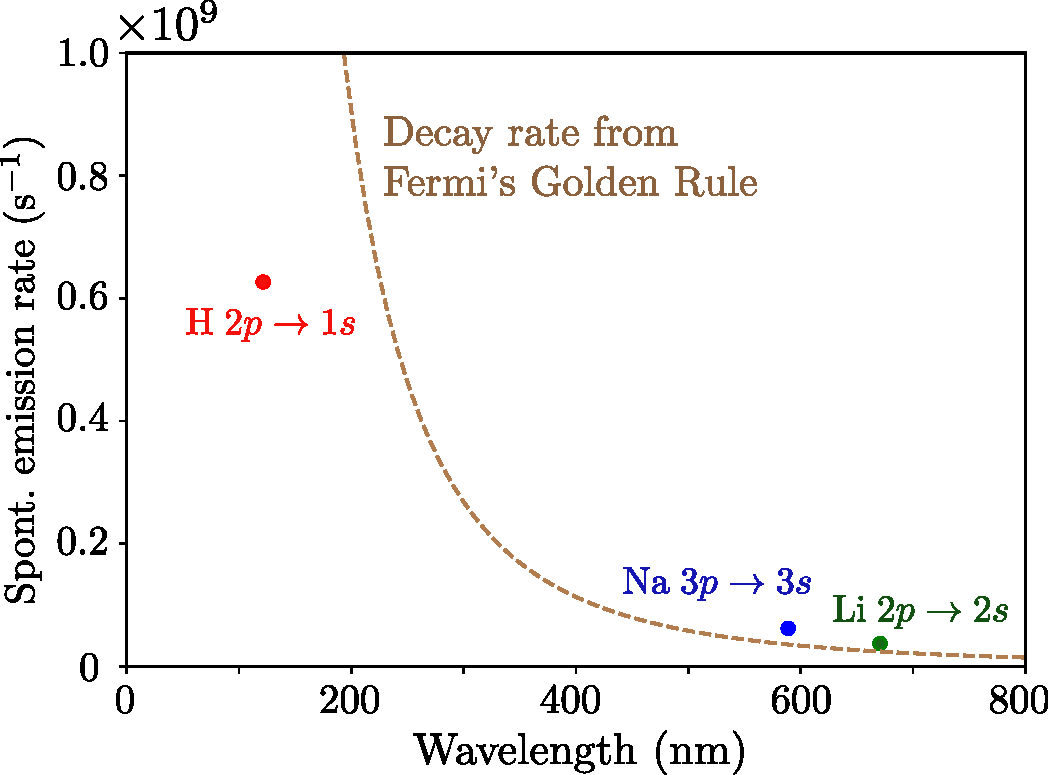
\includegraphics[width=0.53\textwidth]{emissionrates}
  \caption{Spontaneous emission rates (Einstein $A$ coefficients) for
    the $2p\rightarrow 1s$ transition in hydrogen, the
    $2p\rightarrow2s$ transition in lithium, and the $3p\rightarrow3s$
    transition in sodium.  Data points extracted from the NIST Atomic
    Spectra Database
    (\href{https://www.nist.gov/pml/atomic-spectra-database}{https://www.nist.gov/pml/atomic-spectra-database}).
    The dashed curve shows the decay rate based on Fermi's Golden
    Rule, with $|\mathbf{d}| \approx 10^{-10}\,\mathrm{m}$.  }
\end{figure}

%% Need to treat both electrons and photons on the same footing, with QFT
%% language.  Renormalization.

\section*{Exercises}

\begin{enumerate}
\item
  In Section \ref{sec:em_quantization}, we derived the vector
  potential operator, in an infinite volume, to be
  \begin{equation}
    \hat{\mathbf{A}}(\mathbf{r},t) = \int d^3k \sum_{\lambda} 
  \sqrt{\frac{\hbar}{16\pi^3\epsilon_0\omega_{\mathbf{k}}}}\,
  \Big(\hat{a}_{\mathbf{k}\lambda} \, e^{i(\mathbf{k}\cdot\mathbf{r} - \omega_{\mathbf{k}} t)}
  + \mathrm{h.c.}\Big)\, \mathbf{e}_{\mathbf{k}\lambda}.
  \end{equation}
  Since $[\hat{a}_{\mathbf{k}\lambda},
    \hat{a}^\dagger_{\mathbf{k}'\lambda'}] =
  \delta^3(\mathbf{k}-\mathbf{k}') \delta_{\lambda\lambda'}$, the
  creation and annihilation operators each have units of $[x^{3/2}]$.
  Prove that $\hat{\mathbf{A}}$ has the same units as the classical
  vector potential.

\item Repeat the spontaneous decay rate calculation from
  Section~\ref{sec:decay} using the finite-volume versions of the
  creation/annihilation operators and the vector potential operator
  \eqref{Aoperator}.  Show that it yields the same result
  \eqref{alpha}.
  \label{ex:alpha_finite}

\item
  The density of photon states at energy $E$ is defined as
  \begin{equation}
    \mathcal{D}(E) = 2\int d^3k\; \delta(E-E_{\mathbf{k}}),
  \end{equation}
  where $E_{\mathbf{k}} = \hbar c |\mathbf{k}|$.  Note the factor of 2
  accounting for the polarizations.  Prove that
  \begin{equation}
    \mathcal{D}(E) = \frac{8\pi E^2}{\hbar^3c^3},
  \end{equation}
  and show that $\mathcal{D}(E)$ has units of $[E^{-1}V^{-1}]$.
  \label{ex:DE}

\end{enumerate}

\section*{Further Reading}

\begin{enumerate}[[1{]}]
\item F.~J.~Dyson, \textit{1951 Lectures on Advanced Quantum Mechanics
  Second Edition}, arxiv:quant-ph/0608140. [\href{https://arxiv.org/abs/quant-ph/0608140}{link}]
\label{cite:dyson}

\item A.~Zee, \textit{Quantum Field Theory in a Nutshell} (Princeton
  University Press, 2010).
\label{cite:zee}

\item L.~L.~Foldy and S.~A.~Wouthuysen, \textit{On the Dirac Theory of
  Spin $1/2$ Particles and Its Non-Relativistic Limit}, Physical
  Review \textbf{78}, 29 (1950). [\href{https://journals.aps.org/pr/abstract/10.1103/PhysRev.78.29}{link}]
\label{cite:foldy}
\end{enumerate}

\end{document}


%% For decades after the discovery of quantum mechanics, the quantum
%% double-slit experiment was just a ``thought experiment'', meant to
%% illustrate the features of quantum mechanics that had been uncovered
%% by other, more complicated experiments.  Nowadays, the most convenient
%% way to do the experiment is with light, using single-photon sources
%% and single-photon detectors.  Quantum interference has also been
%% demonstrated experimentally using electrons, neutrons, and even
%% large-scale particles such as buckyballs.
